% Mirror: https://github.com/SIGma-UIUC/presentation-format
% --------------------------------------------------------------------
% This is a simple Beamer document that uses beamerthemesigma.sty
% Reading the comments should help you create a presentation even if
% you've never used Beamer before.
% --------------------------------------------------------------------

% Set our document class to Beamer
\documentclass[aspectratio=169, handout]{beamer}

% Some packages for nice font encodings in the final PDF
\usepackage[utf8]{inputenc}
\usepackage[T1]{fontenc}

% From Jeff E
\usepackage{algo}

% Some more macros
\usepackage{sigmastyle}

% Citations
\usepackage{cite}

% To insert images
\usepackage{graphicx}

% To insert gifs
\usepackage{animate}

% Useful packages from the AMS
\usepackage{amsmath,amssymb,amsthm}

% Package for code highlighting
\usepackage{minted}
\setminted{linenos=true, breaklines=true, breakanywhere=true, style=default}
\usemintedstyle{monokai}

% Set a title
\title{Clique Clustering}
\subtitle{The K-clique Percolation Method}

% Set a subtitle if you desire
%\subtitle{\cite[Chapter~7]{TAOCP4A} and \cite[Chapter~7.2.2.1]{TAOCP4B}}

% Whoever worked on the presentation:
\author{Phil}

% An institute name, if you're so inclined
% \institute{University of Illinois Urbana-Champaign}

% Use the SIGma theme for this Beamer presentation
\usetheme{sigma}
% --------------------------------------------------------------------

% Begin document
\begin{document}

% Beamer calls each slide a "frame", defined within the environment:
% \begin{frame}
%   <frame content here>
% \end{frame}

% This frame is just the title.
\begin{frame}
\titlepage
\end{frame}

\date{}

% A frame with the table of contents.
% This frame's title is "Outline".
\begin{frame}{Outline}
  \tableofcontents
\end{frame}

\section{Percolation}
\frame{\sectionpage}
\begin{frame}{Percolating Water Problem}
\begin{itemize}
    \item Assume that some liquid is poured on top of some porous material. Will the liquid be able to make its way from hole to hole and reach the bottom?
    \begin{itemize}
        \pause
        \item \textcolor{sigma@mainblue}{Model:} three-dimensional network of $n \cross n \cross n$ vertices, usually called "sites", in which the edge or "bonds" between each two neighbors may be open or closed
        \pause
        \item \textcolor{sigma@mainblue}{Probabilistic:} A bond is open with probability $p$ and closed $1-p$.
    \end{itemize}
    \pause
    \item For a given $p$, what is the probability that an open path exists from the top to the bottom?
\end{itemize}
\end{frame}

\begin{frame}{Below 50\% Openness}
\begin{figure}
\centering
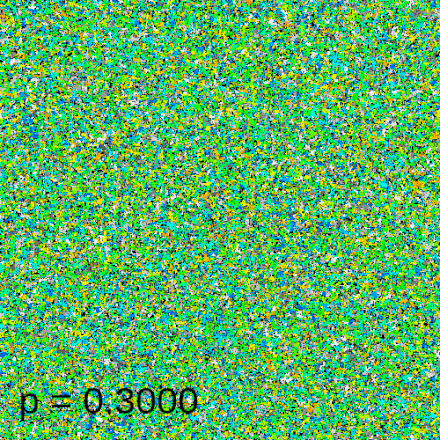
\includegraphics[scale=0.22]{percolation-gif/percolation-1-0.png}
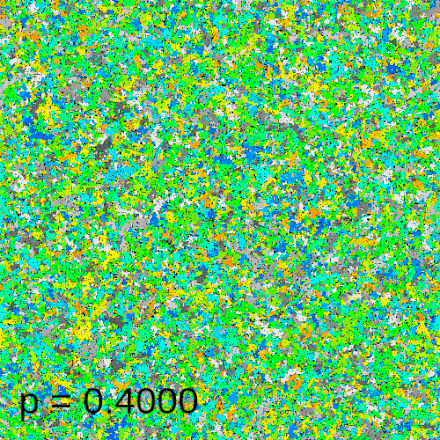
\includegraphics[scale=0.22]{percolation-gif/percolation-1-20.png}
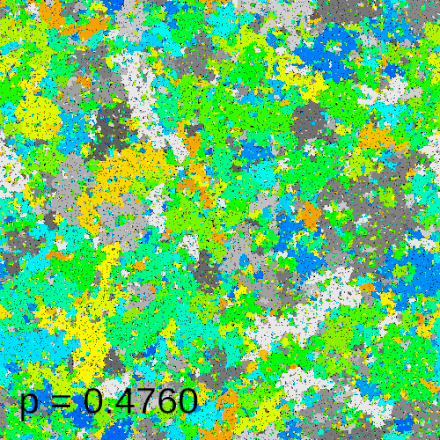
\includegraphics[scale=0.22]{percolation-gif/percolation-1-40.png}
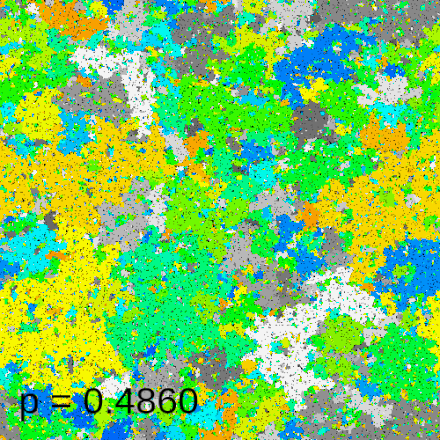
\includegraphics[scale=0.22]{percolation-gif/percolation-1-50.png}
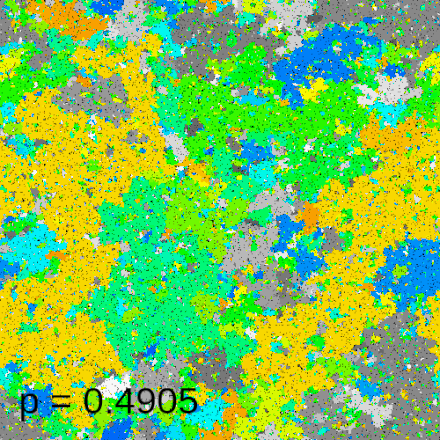
\includegraphics[scale=0.22]{percolation-gif/percolation-1-55.png}
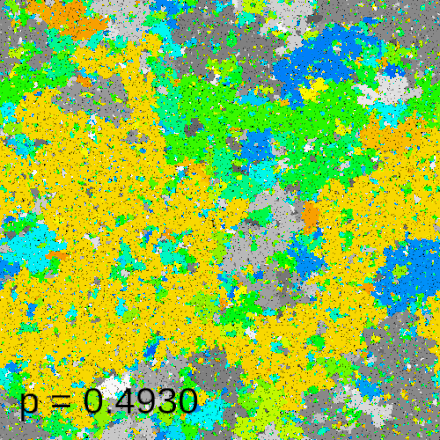
\includegraphics[scale=0.22]{percolation-gif/percolation-1-60.png}
\end{figure}
\end{frame}

\begin{frame}{Above 50\% Openness}
\begin{figure}
\centering
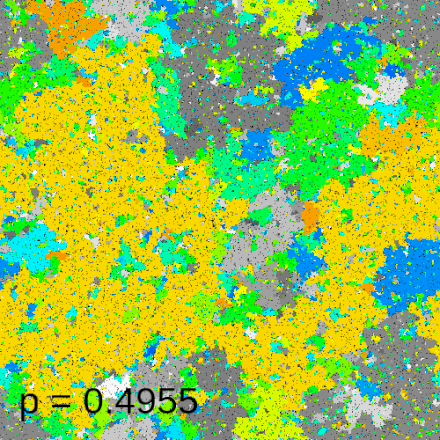
\includegraphics[scale=0.22]{percolation-gif/percolation-1-65.png}
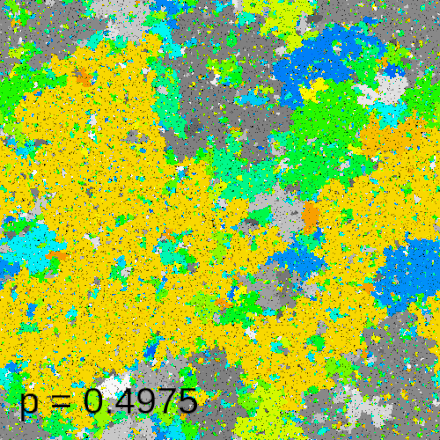
\includegraphics[scale=0.22]{percolation-gif/percolation-1-69.png}
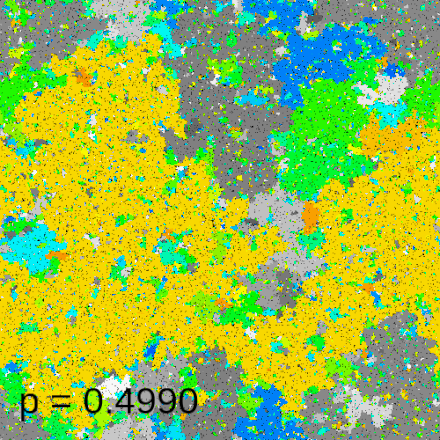
\includegraphics[scale=0.22]{percolation-gif/percolation-1-72.png}
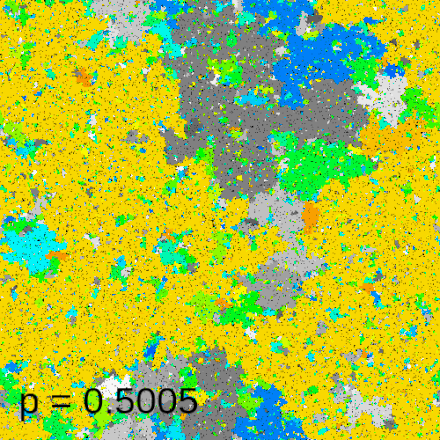
\includegraphics[scale=0.22]{percolation-gif/percolation-1-75.png}
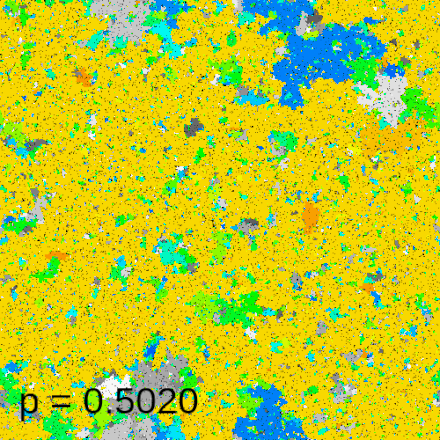
\includegraphics[scale=0.22]{percolation-gif/percolation-1-78.png}
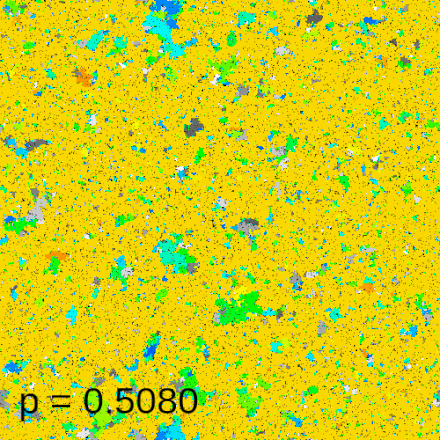
\includegraphics[scale=0.22]{percolation-gif/percolation-1-90.png}
\end{figure}
\end{frame}

\section{The Phase Transition™}
\frame{\sectionpage}

\begin{frame}{New Topic: Random Graphs \cite{ERgraph}}
\begin{itemize}
\item \textcolor{sigma@mainblue}{Idea:} Define some parameters and generate a graph probabilistically
\pause
\item \textcolor{sigma@mainblue}{Erdős–Rényi Model:} The most common model
\item $G(n,p)$: Add $n$ nodes, then add edges with probability $p$
\item $G(n,M)$: Add $n$ nodes, then pick uniformly from all configurations of $M$ edges
\end{itemize}
\end{frame}

\begin{frame}{The "Percolated" Graph}
\begin{itemize}
\item The ER graph's definition is closely related to the percolation problem defined earlier
\pause
\item \textbf{G(n,p):} each edge has a fixed probability of being present or absent, independently of the other edges
\pause
\item \textbf{An ER graph also has a percolation constant!}
\pause
\item The evolution of the ER graph structure with increasing $p$ can be very precisely proven [not in this presentation] but it is dominated by the same critical percolation constant of $p = \frac{1}{n}$
\end{itemize}
\end{frame}

\begin{frame}{Erdős–Rényi Phase Transition: $p = 75\% \frac{1}{n}$}
\begin{figure}
\centering
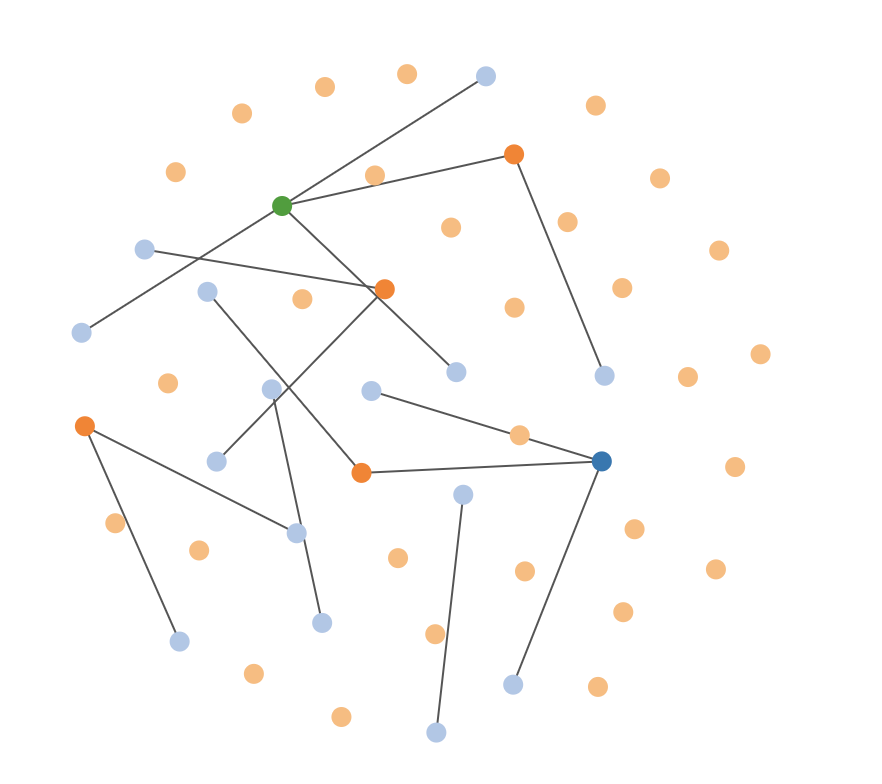
\includegraphics[scale=0.22]{images/percolation-2-1.png}
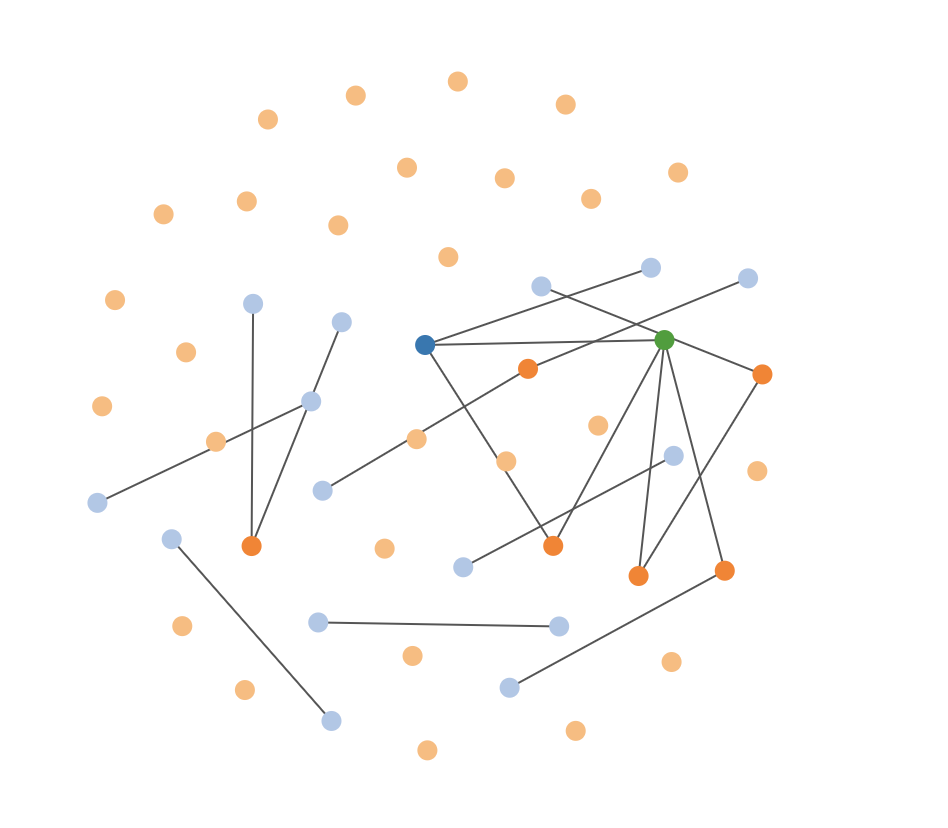
\includegraphics[scale=0.22]{images/percolation-2-2.png}
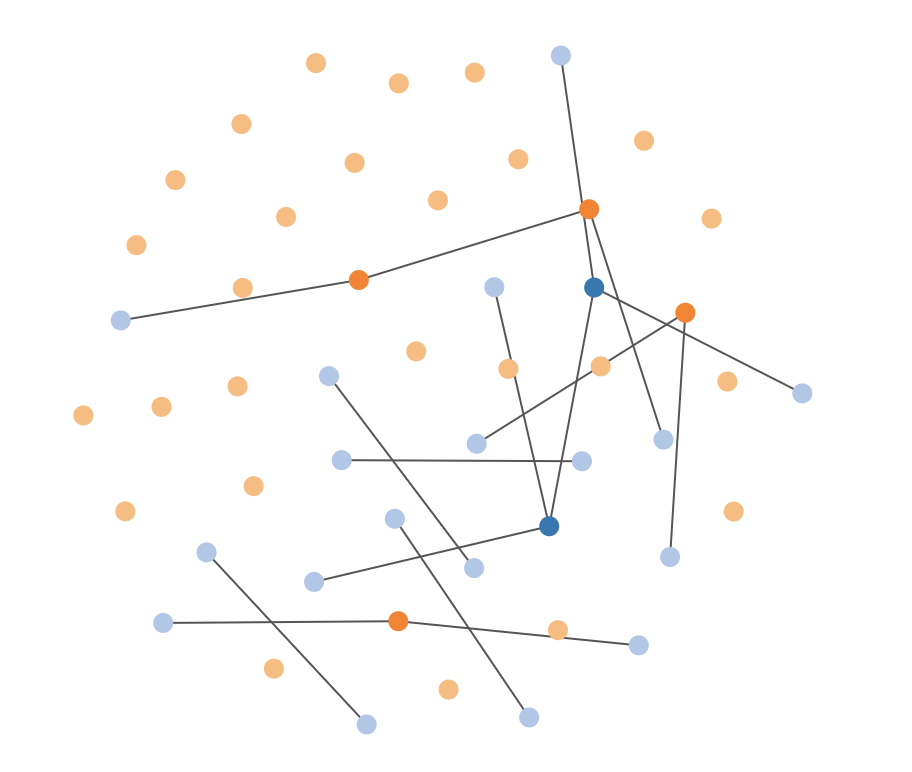
\includegraphics[scale=0.22]{images/percolation-2-3.png}
\end{figure}
\end{frame}

\begin{frame}{Erdős–Rényi Phase Transition $p = 125\% \frac{1}{n}$}
\begin{figure}
\centering
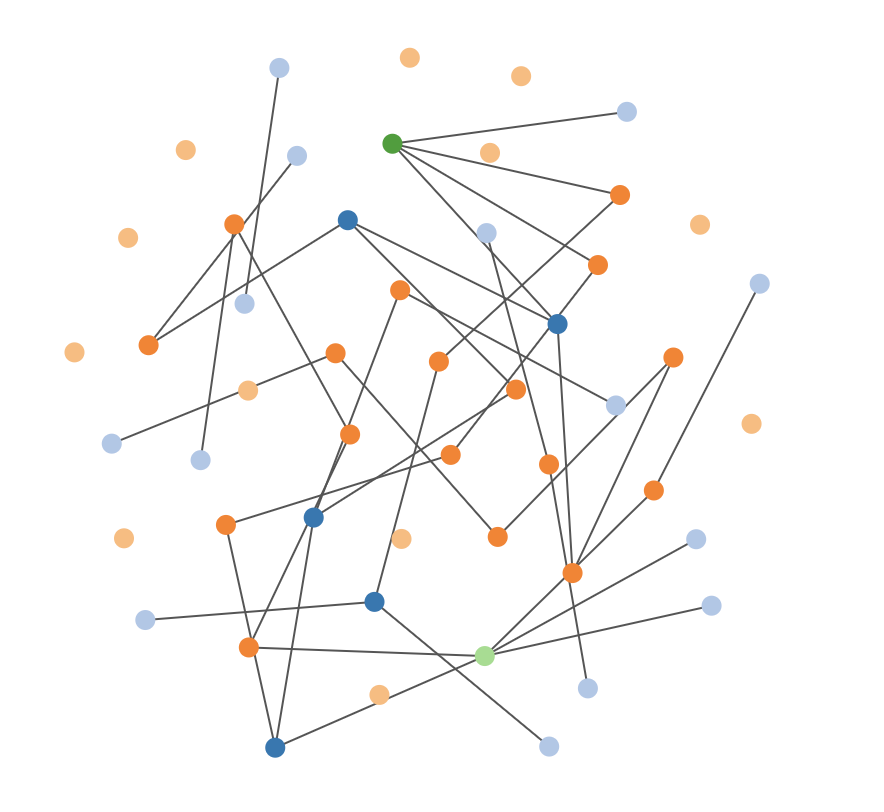
\includegraphics[scale=0.22]{images/percolation-3-1.png}
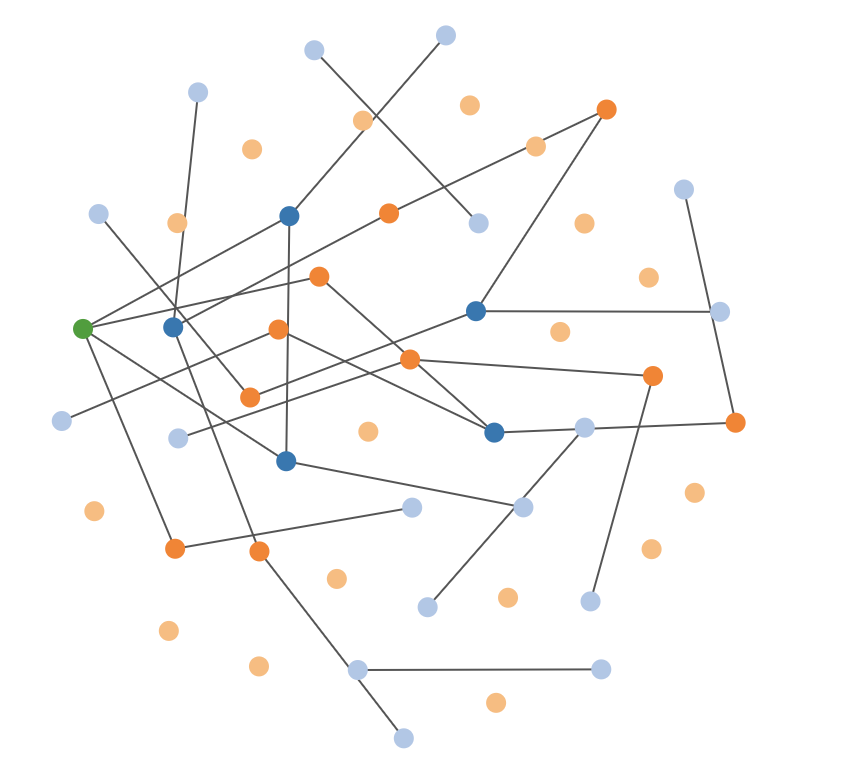
\includegraphics[scale=0.22]{images/percolation-3-2.png}
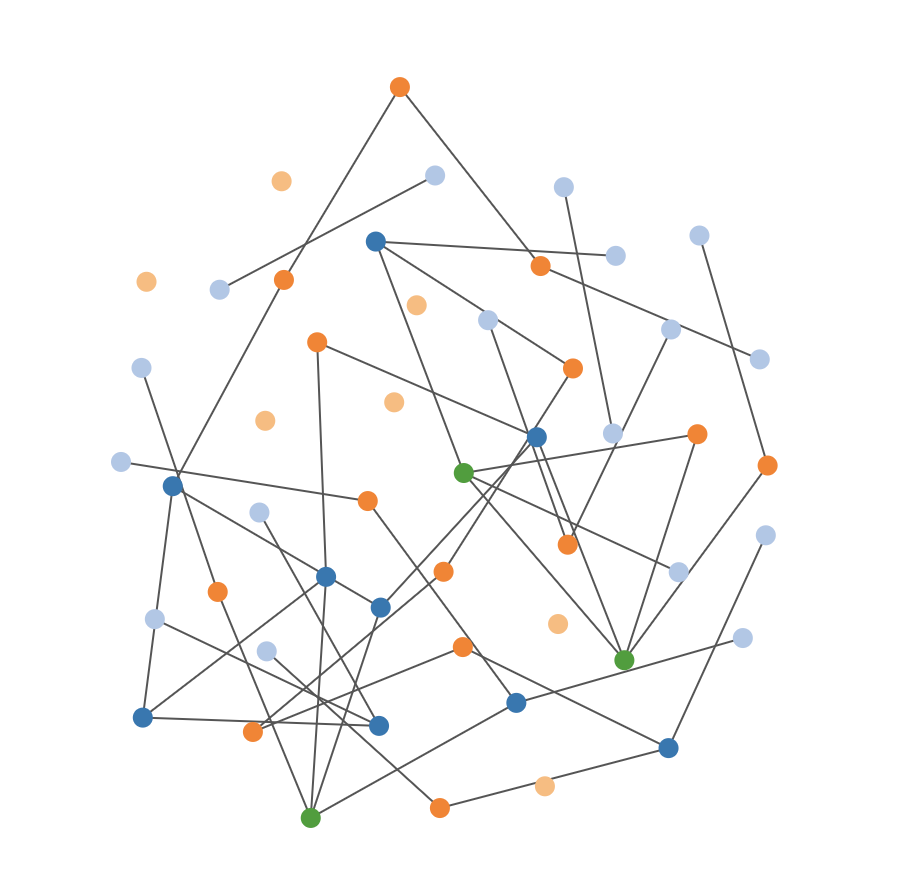
\includegraphics[scale=0.22]{images/percolation-3-3.png}
\end{figure}
\end{frame}

\begin{frame}{Generalizing}
\begin{itemize}
\item The giant connected component is made up of nodes connected to \textit{each other}
\pause
\item The giant connected component is made up of pairs of nodes connected to \textbf{other, possibly overlapping pairs of nodes}
\pause
\item Can we find denser "clusters" by finding \textbf{cliques} connected to other cliques? \textbf{Yes!}
\end{itemize}
\end{frame}

\section{Cliques}
\frame{\sectionpage}
\begin{frame}{Cliques Review}
\begin{figure}
\centering
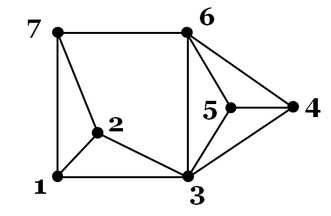
\includegraphics[scale=0.3]{images/clique-1.png}
\end{figure}
\begin{itemize}
\item Some definitions for review:
\pause
\item \textit{Definition:} A clique $c$ is a fully connected set of nodes, i.e.
every pair of its vertices is connected by a link in the graph.
\item \textit{Definition:} A $k$-clique $c_k$ is a clique of $k$ nodes.
\item \textit{Definition:} Two $k$-cliques are said to be adjacent if
and only if they share $k-1$ nodes.
\end{itemize}
\end{frame}

\begin{frame}{CPM Community}
\begin{figure}
\centering
\only<1,2,3,4>{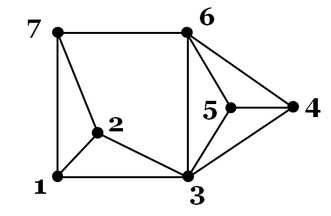
\includegraphics[scale=0.3]{images/clique-1.png}}
\only<5>{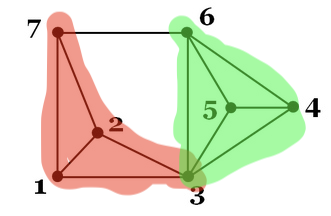
\includegraphics[scale=0.3]{images/clique-2.png}}
\end{figure}
\begin{itemize}
\item \textit{Definition:} A "clique percolation method" community is defined as the maximal union of k-cliques that can be reached from each other through a series of adjacent k-cliques
\item How do we intuit what this means?
\pause
\item Start with a clique "template", and "roll it over" on the graph. \{1, 2, 7\} rolls over to \{1, 2, 3\}
\pause
\item Alternatively, the "Group Chat of Theseus": take one node out of the clique, include a new one.
\pause
\item Where are the 3-clique communities on this graph?
\pause
\end{itemize}
\end{frame}

\begin{frame}{}
      \begin{center}
    {\color{sigma@mainblue} \LARGE Questions?}
  \end{center}
\end{frame}

\section{Clique Percolation Algorithm}
\frame{\sectionpage}

\begin{frame}{Motivation}
\begin{itemize}
\item We want to understand the structure of a graph - the "communities" within it
\begin{itemize}
\item ex. social media - what topics or communities someone participates in or follows
\item ex. biology - identify related proteins within an interaction network
\end{itemize}
\pause
\item Our approach (overlapping cliques) is an intuitive and deterministic definition of a community
\item Allows for overlapping communities - many other methods don't do this
\item Density requirement is freely adjustable via $k$
\end{itemize}
\end{frame}

\begin{frame}{Algorithm Requirements}
\begin{itemize}
\item \textit{Subtask:} find the cliques
\begin{itemize}
\item Either find all maximal cliques, or find all $k$-cliques in a graph
\item These are both NP-hard problems! Outside the scope of this lecture
\item A recent CPM paper uses a parallelized algorithm \cite{KClique}
\end{itemize}
\pause
\item \textit{Subtask:} storing the communities / connected components
\begin{itemize}
\item We will use a \textbf{Union-Find data structure} (disjoint sets)
\item UF.MakeSet(): creates a new tree with one node $p$, corresponding to a new empty
set, and returns $p$.
\item UF.Find(p) returns the root of the tree
\item UF.Union($r_1, ..., r_l$): performs the union of trees represented by their roots $r_i$ by making one root the parent of all others.
\end{itemize}
\end{itemize}
\end{frame}

\begin{frame}{Pseudocode}
\begin{nalgo}
    \underline{\textsc{Basic CPM algorithm}(\emph{G})}:
    \\\label{}  \textsc{UF} $\gets$ Union-Find data structure
    \\\label{}  \textsc{Dict} $\gets$ \Left[\Right]
    \\\label{}  \textbf{for} each $k$-clique $c_k \in  G$ \textbf{do}:\+
    \\\label{communities of $c_k$ to merge}    $S \gets \{\}$
    \\\label{}    \textbf{for} each $(k-1)$-clique $c_{k-1} \subset c_k$ \textbf{do}:\+
    \\\label{}      \textbf{if} $c_{k-1} \in$ \textsc{Dict.keys()} \textbf{then}\+
    \\\label{}        $p \gets$ \textsc{UF.Find(Dict[$c_{k-1}$])}\-
    \\\label{}      \textbf{else}\+
    \\\label{}        $p \gets$ \textsc{UF.MakeSet()}
    \\\label{}        \textsc{Dict[$c_{k-1}$]} \gets $p$\-
    \\\label{}        $S \gets S \cup \{p\}$\-
    \\\label{}        \textsc{UF.Union($S$)}
    \end{nalgo}
\end{frame}

\begin{frame}{}
      \begin{center}
    {\color{sigma@mainblue} \LARGE Questions?}
  \end{center}
\end{frame}

\section{Addenda}
\frame{\sectionpage}

\begin{frame}{Percolation Threshold}
\begin{itemize}
\item There are also threshold thresholds for clique communities. What edge probability $p$ is the threshold to producing one giant connected community in an ER graph?
\pause
\item Intuition: going back to the "rolling-over" analogy. Within a "rolling", at the threshold, there should be, in expectation, one adjacent clique at each clique, to "continue" to build the cluster.
\pause
\item $(k-1) \times (N - k - 1) p_c^{k-1} = 1$: candidate vertices to remove $\times$ candidate vertices to add
\item For large $N$, this comes out to $N(k-1) p_c^{k-1} = 1$ \cite{CPM05}
\pause
\end{itemize}
\begin{align}
p_c(k) = \frac{1}{\Left[ N(k-1) \Right]^{\frac{1}{k-1}}}
\end{align}
\end{frame}

\begin{frame}{Optimizations}
\begin{itemize}
\item The given CPM algorithm is prohibitively expensive in memory because we store large number of $(k-1)$-cliques
\item \textit{Optimization:} instead of disjoint sets of $(k-1)$ cliques, consider non-disjoint sets of $z$-cliques s.t. $z < (k-1)$ \cite{CPMmem}
\pause
\item why are there fewer $z$-cliques? Consider binomial theorem, $k \ll M$
\item this leads to an \textit{approximation} of the previous algorithm, but it is otherwise very similar and produces very similar results
\end{itemize}
\end{frame}

%\section{Review of Exact Cover}
%\frame{\sectionpage}
%\begin{frame}{Exact Cover Problems}
%\begin{itemize}
%    \item The goal of Exact Cover is to select subsets of some list of items according to certain criterion: \pause
%    \begin{itemize}
%        \item \textcolor{sigma@mainblue}{Cover:} Select subsets such that their \textbf{union} is all items
%        \item \textcolor{sigma@mainblue}{Exact:} Each item is in \textbf{exactly one} subset
%    \end{itemize} \pause
%    \item In 1972, Richard Karp proved that Exact Cover, among 20 other problems, is \textcolor{sigma@mainblue}{NP-%Complete}
%        \begin{itemize}
%            \item Easy to verify solutions in polynomial time
%            \item Hard to solve, best known solutions run in exponential time 
%            \item Can simulate (or reduce) other problems in NP using Exact Cover
%        \end{itemize}
%\end{itemize}
%\end{frame}


%\begin{frame}{An Example of Exact Cover}
%    \textcolor{sigma@mainblue}{\textbf{Goal:}} Select rows such that each column in the selection has one $1$
%    \[
%        \begin{pmatrix}
%            1 & 0 & 1 & 0 & 0  \\
%            0 & 0 & 0 & 0 & 1  \\
%            0 & 1 & 0 & 1 & 0  \\
%            0 & 0 & 1 & 0 & 1  \\
%            1 & 0 & 1 & 1 & 0  \\
%        \end{pmatrix}
%    \] \pause 
%    We can abstract this to \textcolor{sigma@mainblue}{\underline{options}} containing \textcolor{sigma@mainblue}%{\underline{items}}
%    \begin{table}[]
%        \begin{tabular}{ l l l }
%            $1\colon \bqty{a, c}$& $2\colon \bqty{e}$ & $3\colon \bqty{b, d}$ \\ 
%            $4\colon \bqty{c, e}$ & $5\colon \bqty{a, c, d}$ & \\ 
%        \end{tabular}
%    \end{table} \pause
%    \textcolor{sigma@mainblue}{\textbf{Answer:}} Select options 1, 2, and 3
%\end{frame}

%\begin{frame}{Recursively Solving Exact Cover Problems}
%    In trying to solve the previous problem, you may have naturally found a recursive algorithm to find a solution %\pause
%    \begin{nalgo}
%    \underline{\textsc{FindCover}(\emph{Options, Items, Cover}, $i$)}:
%    \\\label{}  \textbf{if} \emph{Cover} is a cover:\+
%    \\\label{}      \textbf{terminate} successfully\-
%    \\\label{}  \textbf{if} no option in \emph{Options} contains $i$:\+
%    \\\label{}      \textbf{terminate} unsuccessfully\-
%    \\\label{}
%    \\\label{}  $I \gets$ options in \emph{Options} that contain $i$
%    \\\label{}  \emph{Options} $\gets$ \emph{Options} $\setminus I$
%    \\\label{}  \textbf{for} each $O$ in $I$:\+
%    \\\label{}      $j \gets$ an item still not covered
%    \\\label{}      \textsc{FindCover}(\emph{Options}, \emph{Cover} $\cup \set{O}$, $j$)
%    \end{nalgo}
%\end{frame}


%\section{Data Structure}
%\frame{\sectionpage}

%\begin{frame}{}
%    \begin{figure}
%        \centering
%        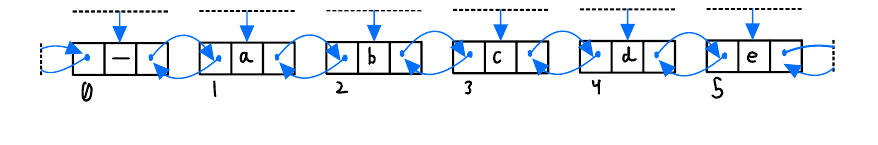
\includegraphics[scale=0.75]{images/Algorithm_X-01-cropped.png}
%    \end{figure}
%    \begin{itemize}
%        \item We create a linked list of our \textcolor{sigma@mainblue}{\textit{items}}, where each %\textcolor{sigma@mainblue}{\textit{item}} will connect to a linked list representing its \textcolor{sigma@mainblue}%{\textit{options}} 
%    \end{itemize}
%\end{frame}

%{
%\usebackgroundtemplate{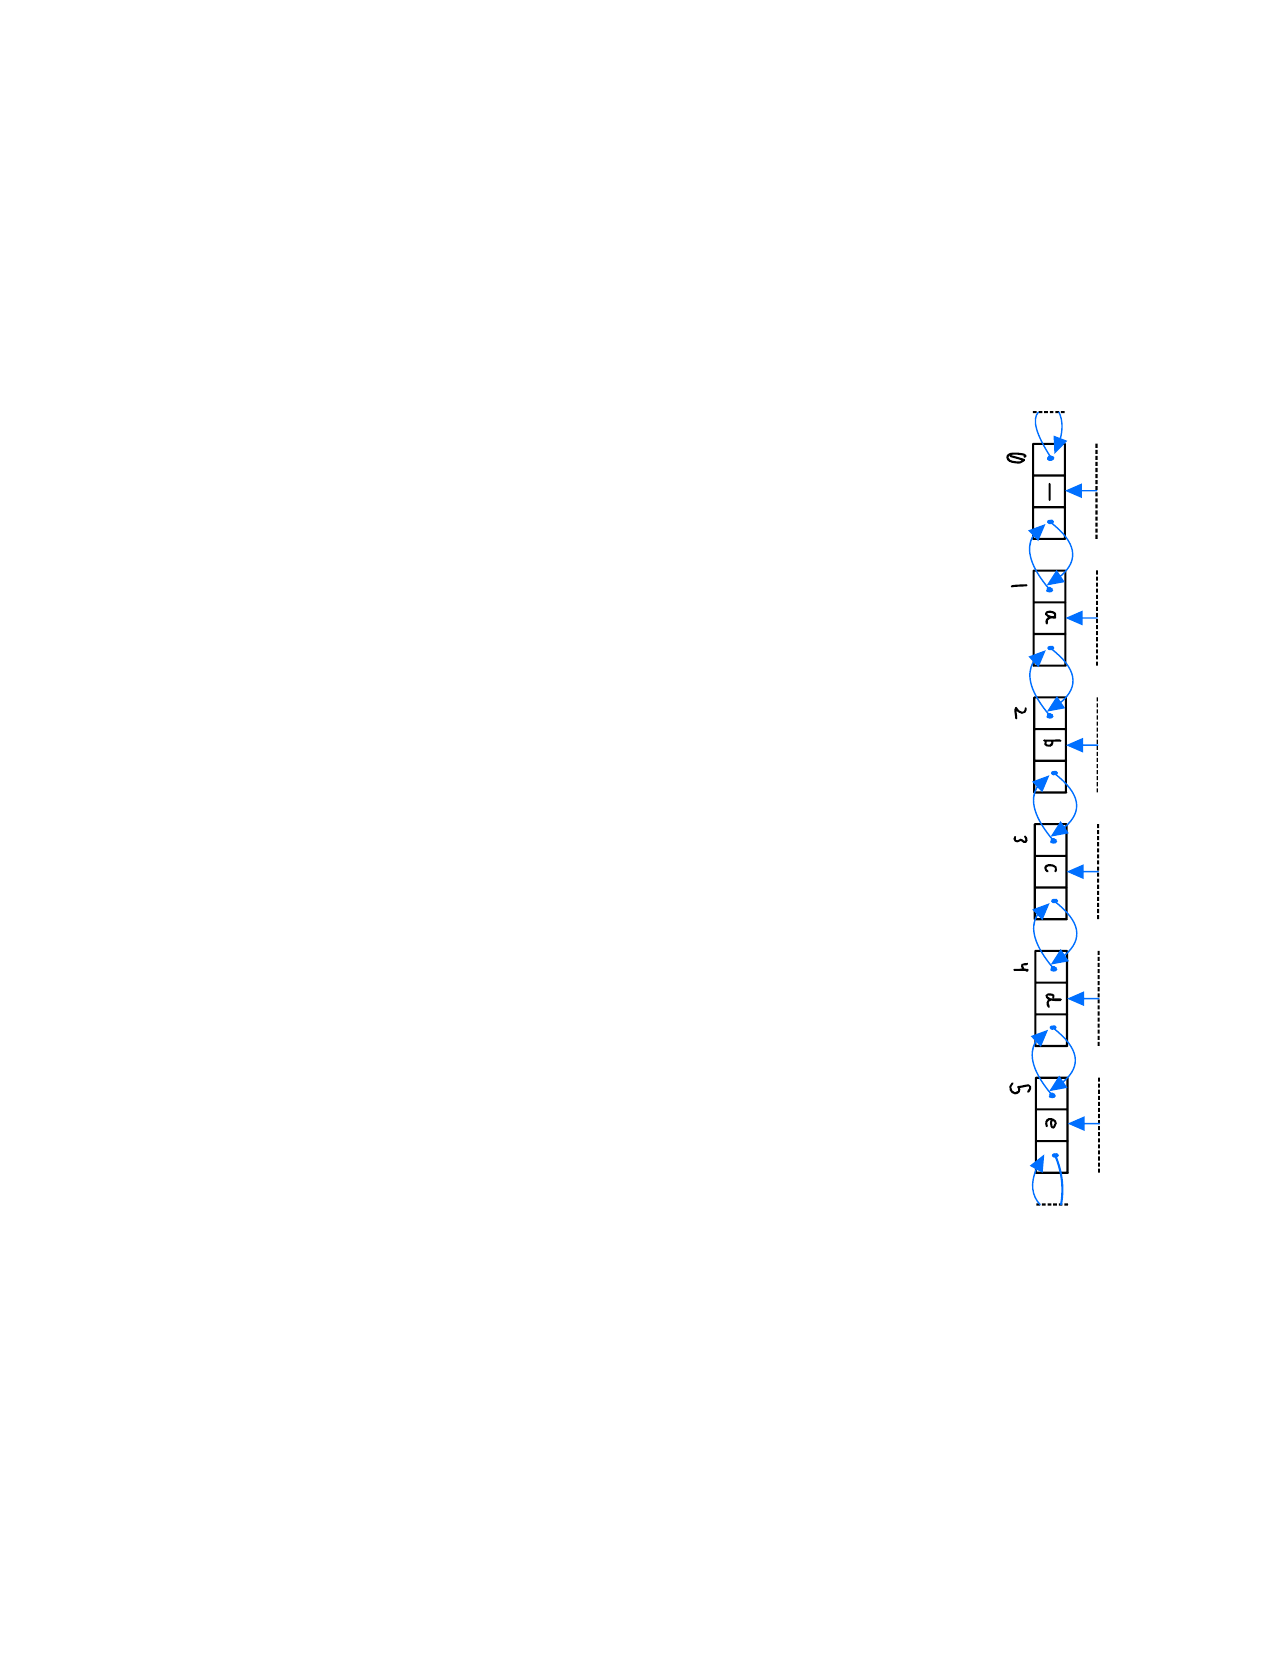
\includegraphics[angle=90,origin=c,scale=0.525]{images/Algorithm_X-01.png}}
%\frame{}
%}

%have you ever wondered: what if a linked list was actually SEVERAL linked lists, all of which were circular and had both up, down, left, AND right links? :D


\begin{frame}{}
      \begin{center}
    {\color{sigma@mainblue} \LARGE Questions?}
  \end{center}
\end{frame}

% \font\eightss=cmssq8
% \font\eightssi=cmssqi8
% \newcommand\quoteAuthorDate[3]{\begingroup
%   \baselineskip 10pt
%   \parfillskip 0pt
%   \interlinepenalty 10000 % not needed in example
%   \leftskip 0pt plus 40pc minus \parindent
%   \let\rm=\eightss
%   \let\sl=\eightssi
%   \everypar{\sl}#1\par
%   \nobreak\smallskip
%   \noindent\rm--- #2\unskip\enspace(#3)\par
%   \endgroup}
% % If someone can figure out how to horizontally center this and make the text bigger that'd be cool
% \begin{frame}
%     \begin{center}
%         \item \quoteAuthorDate{Combinatorics is special. Most mathematical topics which can be covered in a lecture course build towards a single, well-defined goal, such as the Prime Number Theorem. Even if such a clear goal doesn’t exist, there is a sharp focus (e.g. finite groups). By contrast, combinatorics appears to be a collection of unrelated puzzles chosen at random. Two factors contribute to this. First, combinatorics is broad rather than deep. Second, it is about techniques rather than results.}{PETER J. CAMERON}{\color{sigma@mainblue}1995}
%     \end{center}
% \end{frame}

% Remove this slide if you came up with all the material yourself
\begin{frame}{Bibliography}
    \bibliographystyle{alpha}
    {\scriptsize \bibliography{refs}}
\end{frame}

\end{document}